%set the master document for easy compilation
%!TEX root = ../D3_5_3.tex

  %-----------------------------------------------------------------------
  \section{DMI Controller}
  %-----------------------------------------------------------------------
  %\tbc
  %Valerio D´Angelo/Baseliyos Jacob

  \subsubsection{Reference to the SRS or other Requirements (or other requirements)}

   ERA\_ERTMS\_015560

  \subsubsection{Short description of the functionality}
  The DMI controller interact with the DMI display and is responsible for alls procedures between the DMI display and Driver. Furthermore, the DMI controller will interact with the DMI Management to compute the received information (e.g. driver number request, ...) and send, if necessary, data or reports to the DMI Management (acknowledge, text messages...). The DMI Controller is a passive module, this means that all the processing are performed EVC-side, therefore the DMI Controller simply responds to the requests of the EVC or Driver and performs some checks according with the information received from EVC.

  \begin{figure}
  \centering
  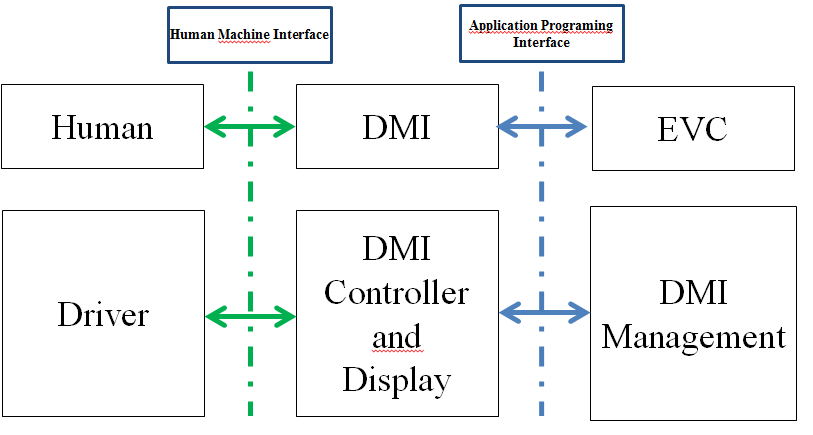
\includegraphics[width=.8\textwidth]{images/DMI_Interfaces}
  \caption{DMI Interfaces}
  \end{figure}

  \subsubsection{Interface}
  The DMI Controller has two interfaces. One between DMI Controller and DMI Display and one between DMI Controller and DMI Management. 
  The structure of the interface between DMI Controller and DMI Display is driven by the logic of SCADE Display therefore It doesn't follow any standard or constraints (It will not be described in this chapter).
  DMI Controller and DMI Management exchange packets. Each packet is a structured type with a valid flag (a boolean variable), the DMI controller takes into account the data inside the packet only when the valid flag is true.

  The interface between DMI Controller and DMI Management consist of three parts according with the direction of the information:
  
  \begin{itemize}
  \item From DMI Management to DMI Controller
  \item From DMI Controller to DMI Management 
  \item Both ways directions (You will find the same type both as input than as output)
  \end{itemize}
  


\paragraph{From DMI Management to DMI Controller}

In the following table are listed the inputs coming from DMI Management with a brief description:\\
  %\begin{table}[H]
    \begin{tabular}{| c | l | l | l | l |}
      \hline
      \textbf{NAME} & \textbf{DESCRIPTION} \\ \hline
      \texttt{DMI\_entry\_request} & Request to input data (e.g. driver id, Train running number etc.)\\
      \texttt{DMI\_identifier\_request} & Request of the DMI informations\\
      \texttt{DMI\_menu\_request} & Request to enable or disable buttons\\
      \texttt{DMI\_dynamic} & Contains informations about current speed, current mode etc.\\
      \texttt{DMI\_text\_message} & Contains predefined or plain text messages\\
      \texttt{DMI\_icons} & Request to display one or more icons in any area\\

      \hline
    \end{tabular} 
  % \caption{Overview of input}
    \label{tbl:DMICtrToDMIMng}
  %\end{table}
  
      Please note: TIU\_trainStatus input is missing in the above table. This is the only input coming directly from TIU and contains the open/close Desk signal. 
    
  \paragraph{From DMI Controller to DMI Management}
  In the following table are listed the outputs directed to DMI Management with a brief description:\\
  %\begin{table}[H]
    \begin{tabular}{| c | l | l | l | l |}
      \hline
      \textbf{NAME} & \textbf{DESCRIPTION} \\ \hline
      \texttt{DMI\_identifier} & Information about DMI (e.g. version, cabin identifier etc.)\\
      \texttt{DMI\_driver\_request} & Driver request or acknowledgement\\
      \texttt{DMI\_train\_data\_ack} & Train data acknowledgement\\
      \texttt{DMI\_status\_report} & The actual status of DMI (keep alive)\\
      \texttt{DMI\_text\_message\_ack} & Text message acknowledgement\\
      \texttt{DMI\_icons\_ack} & Icon acknowledgement\\

      \hline
    \end{tabular} 
  % \caption{Overview of input}
    \label{tbl:DMICtrToDMIMng}
  %\end{table}
    
\paragraph{Both ways direction}
In the following table are listed the outputs/inputs  to/from DMI Management with a brief description:\\
  
  %\begin{table}[H]
    \begin{tabular}{| c | l | l | l | l |}
      \hline
      \textbf{NAME} & \textbf{DESCRIPTION} \\ \hline
      \texttt{DMI\_driver\_identifier} & Contains the default or entered driver identifier\\
      \texttt{DMI\_train\_running\_number} & Contains the default or entered train running number\\
      \texttt{DMI\_train\_data} & Contains the default or entered train data\\
      \hline
    \end{tabular} 
  % \caption{Overview of input}
    \label{tbl:DMICtrToDMIMng}
  %\end{table}
  

\subsubsection{Functional Design Description}
  \textbf{Please note}: \textit{DMI Controller is a project under construction, a lot of features and functionalities are missing, therefore the structure described below is a draft version and will be changing in the future.}
  
  The informations (received and sent) could be divided in two groups: Sporadic and Periodic. The first one are received/sent aperiodically in any time instead the second one are received/sent periodically, with a fixed deadline. Are part of Periodic group the output DM\_status\_report and the input DMI\_dynamic all other are Sporadic. Therefore, the structure of DMI Controller module consists of a first main state machine \textit{CabinSM} (Fig. \ref{fig:CabinSM}) triggered by  a \textit{OpenDesk} signal (from TIU). Inside the \textit{DeskIsOpen} state there are other two state machines :\textit{HandshakeSM} and \textit{DynamicInfoSM} (Fig. \ref{fig:DynSporSM}).
  
  HandshakeSM performs an initial handshake between DMI Controller and DMI Management. Before that, no data has to be sent or received to/from DMI Management. When the transition is fired a DMI\_identifier packet is sent to DMI Management with informations about the DMI (e.g. DMI identifier, DMI name etc.). At this point the DMI Controler is ready to manage the sporadic information (e.g. Enter or revalidate DriverID, Enter or revalidate Train running number etc.). 
  
  The DynamicInfoSM state machine is triggered after the handshake, exactly when  HandshakeSM reaches the  DynInfo\_Activated state. At the time when the transition is fired a signal is emitted (startDMI\_status) and begins a periodic sending of DMI status information (keep alive) to DMI Management. Once reached DynamicInfo\_Active, the DMI Controller is ready to receive and manage the dynamic informations.
  
   \begin{figure} 
      	\centering
      	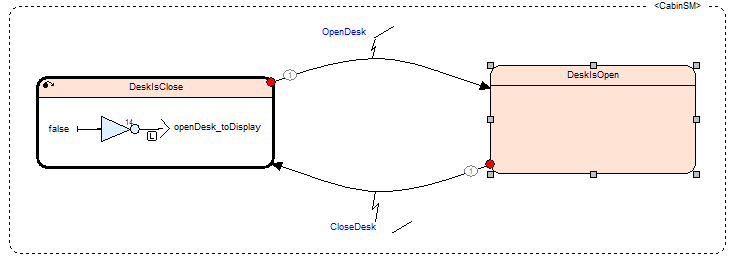
\includegraphics[scale=0.7]{images/CabinSM}
      	\caption{Cabin State Machine.}
      	\label{fig:CabinSM}
   \end{figure}
      
  \begin{figure} 
  \centering
  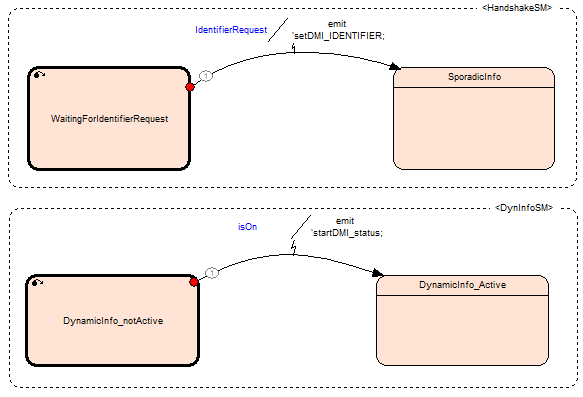
\includegraphics[scale=0.8]{images/DynSporInfoSM}
  \caption{HandshakeSM and DynamicInfoSM State Machines.}
  \label{fig:DynSporSM}
  \end{figure}
  


  With the aim to improve the readability and for a better management of complexity, all the functions (modules, state machines etc.) implemented in each state are divided several diagrams.
  
  The \textit{SporadicInfo} consist of:
  \begin{itemize}
  	\item \textbf{diagram\_SporadicInfo\_Main}: Contains all the modules to manage the sporadic data like ``Enter revalidate Driver ID'', ``Enter or revalidate train running number'', enable buttons in menus. The WindowSM state machine manages the windows that should appear on the DMI(Fig. \ref{fig:win_sm}).
  	
  	\item \textbf{ diagram\_SporadicInfo\_TrainData}: Contains all the logic to store and adapt the incoming train data to a correct visualization on DMI Display.
  	
  	\item \textbf{diagram\_SporadicInfo\_Icon\_Management}: Contains the logic to show/hide one or several icons in area and manage the acknowledgement mechanism if It's required.
  	
  	\item \textbf{ diagram\_SporadicInfo\_DriverID\_TRN}: Contains the logic to store and sent the Train running number and the Driver ID.
  	
  	\item \textbf{diagram\_SporadicInfo\_Text\_Messages}: Contains the modules, state machines and all the logic to manage and display predefined and customized text messages.
  \end{itemize}
  
  The \textit{DynamicInfo\_Active} state consists of:
  \begin{itemize}
  	\item \textbf{diagram\_DynamicInfo\_Main}: Contains modules to store and display the informations like the current mode, ETCS level, RBC connection status and location brake target.
  	\item \textbf{diagram\_SpeedSupervision}: Contains the module where are implemented the behaviour of the speed pointer and the circular speed gauge ( informations about speed target, speed permitted and speed release).
  \end{itemize}
  
  \begin{figure}
  	\centering
  	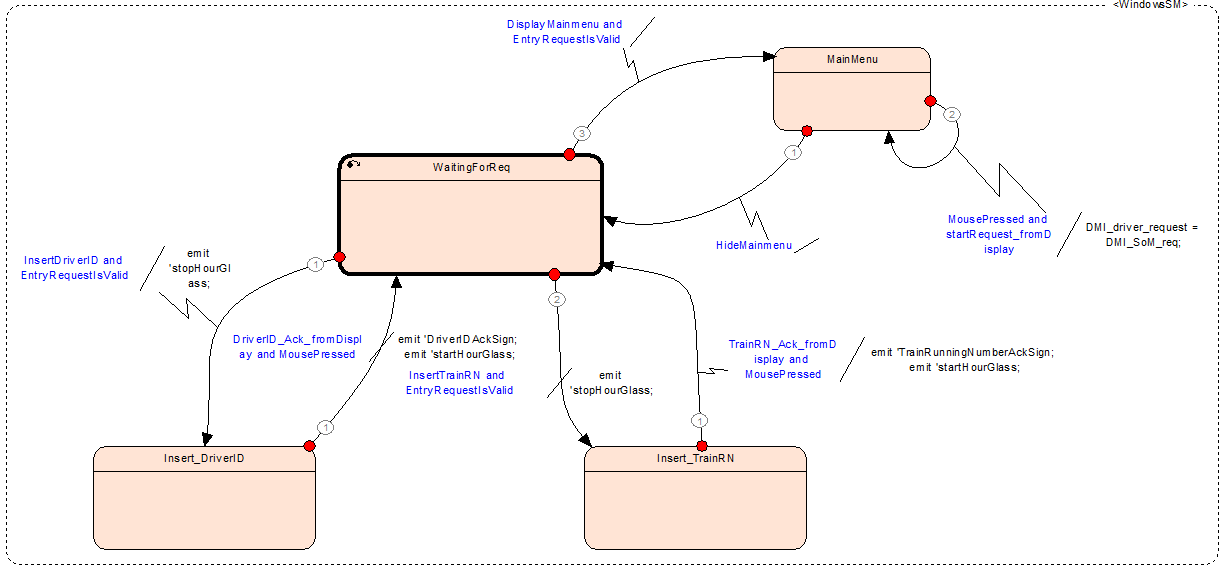
\includegraphics[width=\textwidth]{images/WindowSM}
  	\caption{Windows state machine.}\label{fig:win_sm}
  \end{figure}
  
\subsubsection{Communication Protocol}
This section explains which messages are exchanged among DMI Controller, DMI Management and Start of mission procedure. As mentioned previously the DMI Controller is a passive component, It simply responds to requests, therefore is able to cover different scenarios. Below are some examples.
  
  \paragraph{Start Of Mission scenario} Are detailed, through a sequence diagram, all the activities (exchanged messages) that should be done to start. In this scenario we have three actors: DMI Controller, DMI Management and SoM procedure (the module where is implemented the start of mission procedure). It's assumed that a OpenDesk signal is received and the system starts in Stand By mode (Fig. \ref{fig:SeqDiaSoM}).
 
  \begin{figure}
  \centering
  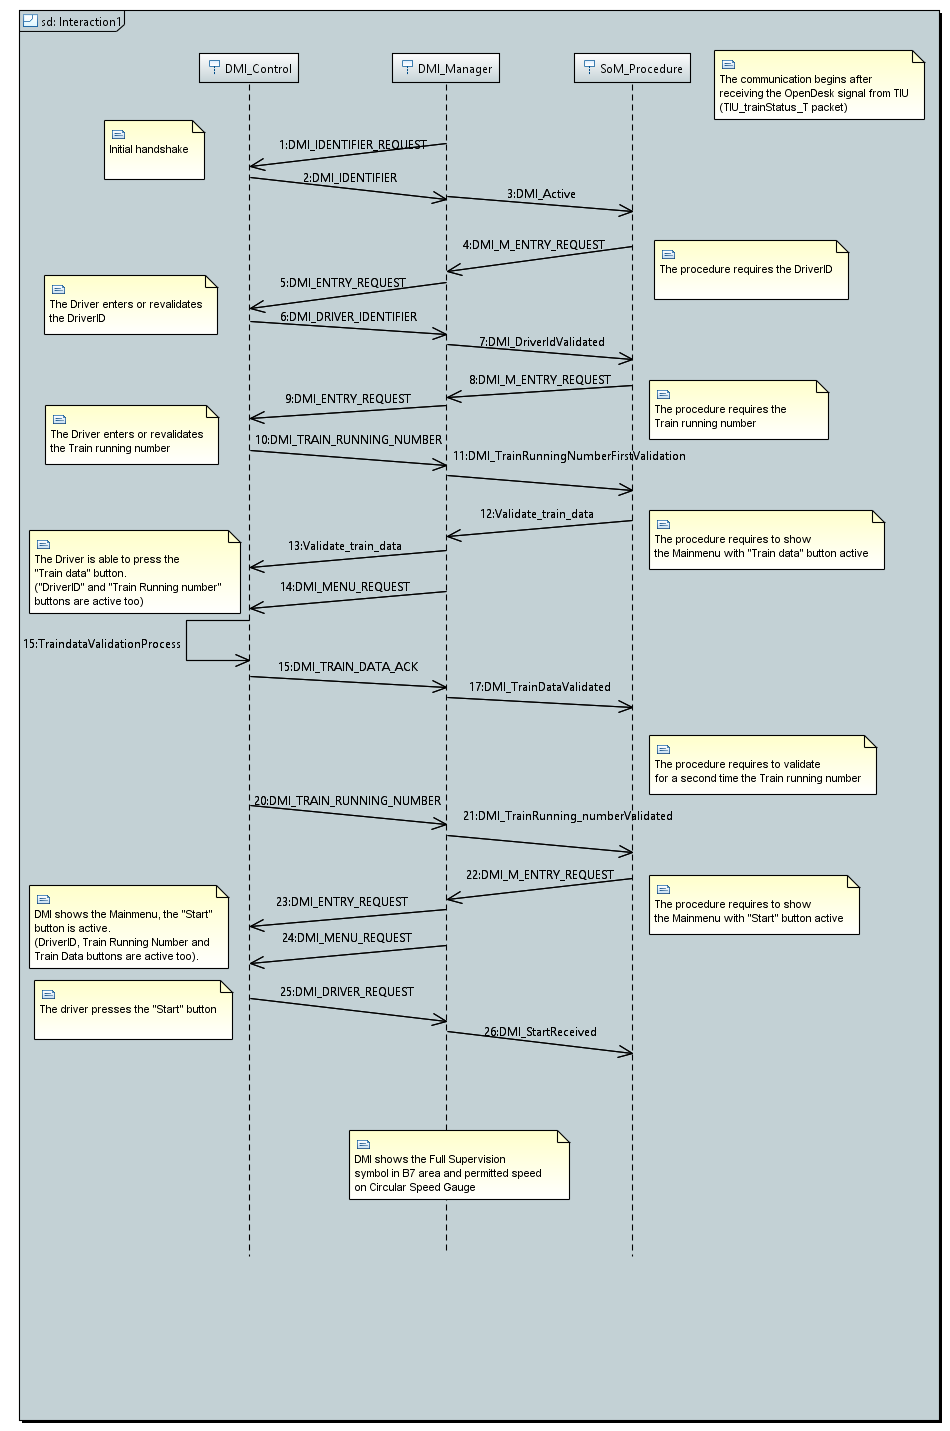
\includegraphics[scale=0.45]{images/SeqDia_DMIctr_DMImng_SoMproc}
  \caption{Sequence Diagram of start of mission scenario}\label{fig:SeqDiaSoM}
  \end{figure}
  

\paragraph{Cyclic Exchange of messages}
The time between two messages has not yet been definitively established, It might change in the future. The DMI status packet implements a keep alive mechanism, this means, if the EVC does not receive any DMI status signal during the lapse time, It shall consider a failure in DMI. This check is not yet implemented.

    \begin{figure}
      \centering
      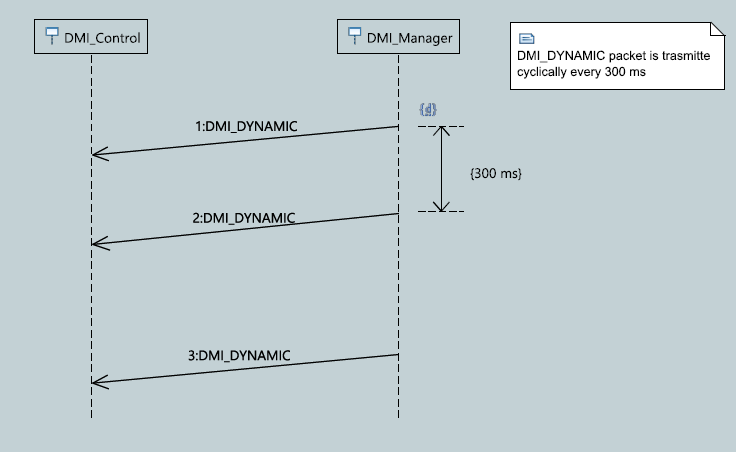
\includegraphics[scale=0.5]{images/DynamicPacket_SeqDia}
      \caption{ Sequence diagram of Dynamic data.}\label{fig:SeqDiaDyn}
    \end{figure}
  
    \begin{figure}
      \centering
      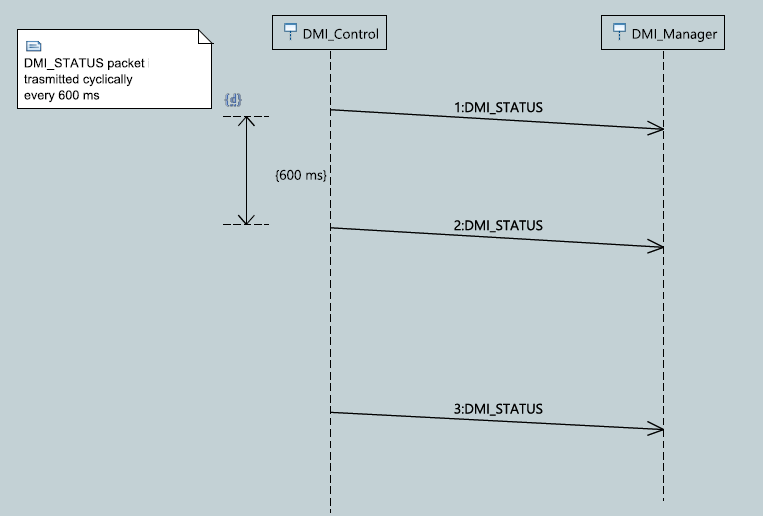
\includegraphics[scale=0.5]{images/DMIStatus_SeqDia}
      \caption{Sequence Diagram of DMI status.}\label{fig:SeqDiaStatus}
     \end{figure}
     

\subsubsection{Reference to the Scade Model}

The SCADE model can be found on github under the following path: \url{https://github.com/openETCS/modeling/tree/master/model/Scade/System/DMI_Control}